\documentclass[handout]{beamer}
\usetheme{Madrid}
\usepackage{pdfpages}
\usepackage[utf8x]{inputenc}
\usepackage{url}
\usepackage{graphicx}
\usepackage{graphics}
\usepackage{adjustbox}
\usepackage{ragged2e}
\usepackage{amsmath, amssymb}
\usepackage{verbatim}
\usepackage{soul}
\usepackage{textpos}
\usepackage{xcolor}
\usepackage{tcolorbox}
\usepackage{lmodern,textcomp}
 \setbeamertemplate{enumerate items}[default]
 \setbeamertemplate{itemize items}[circle]
 \setbeamertemplate{frametitle continuation}{}
\setbeamertemplate{section in toc}[circle]
\setbeamertemplate{subsection in toc}[circle]

\usepackage{tabulary, booktabs}

\usepackage{hyperref}
\hypersetup{
    colorlinks=cyan,
    linkcolor=true,
    filecolor=cyan,      
    urlcolor=cyan,
}

\beamertemplatenavigationsymbolsempty

%%%%%%%%%%%%%%%Color%%%%%%%%%%%%%%%
\definecolor{KIPlum}{HTML}{880052}
\definecolor{box}{RGB}{250, 117, 144}
\usecolortheme[named=KIPlum]{structure}

%%%%%%%%%%%%%%%Bibliography setting%%%%%%%%%%%%%%%
\usepackage[numbers,comma,sort&compress]{natbib}
\makeatletter
\renewcommand{\@biblabel}[1]{#1.} %remove brackets from the ref list
\makeatother



%%%%%%%%%%%%%%%Title page%%%%%%%%%%%%%%%

\title[Applied Epi I: Data Management]{Applied Epidemiology I: Data clearance\\ A review of using Stata}
\date{January 28, 2021}
\author[Enoch Yi-Tung Chen]{Enoch Yi-Tung Chen}
\institute[MEB]{Department of Medical Epidemiology and Biostatistics, Karolinska Insitutet}

%%%%%%%%%%%%%%\begin{document}%%%%%%%%%%%%%%%%

\begin{document}

\begin{frame}
\maketitle 
\end{frame}

%%%%%%%%%%%%%%Ack%%%%%%%%%%%%%%%%
\begin{frame}{Acknowledgements}
This course material is based on my learning from \href{https://staff.ki.se/people/analam}{Anastasia Lam}'s teachings in last year's Applied Epidemiology I lab sessions, and readings from \textit{Epidemiology} by Gordis \cite{Gordis2014}, \textit{A First Course in Probability and Statistics} by Goldsman and Goldsman \cite{Goldsman2020}, \textit{Principles of Biostatistics} by Pagano and Gauvreau \cite{Pagano2000}, and \textit{Biostatistics I} by Gabriel and Frumento \cite{Gabriel2020}. 

I especially want to thank Marlene Stratmann for reviewing the slides and Prof. Paul Dickman for providing me with suggestions to improving the teaching.

\end{frame}


%%%%%%%%%%%%%%Outline%%%%%%%%%%%%%%%%
\section*{Outline}
\begin{frame}{\secname}
 \begin{columns}[t]
        \begin{column}{.5\textwidth}
            \tableofcontents[sections={1-4}]
        \end{column}
        \begin{column}{.5\textwidth}
            \tableofcontents[sections={5-7}]
        \end{column}
\end{columns}
\end{frame}

%%%%
\section{Set up working directory}
\begin{frame}[fragile]{\secname}
\begin{itemize}
 \item<1|handout:1-> 	Working directory is the folder where all your files are stored, and should be set each time you start.
 \item<2|handout:2->  Where is it?
 \item[]<2|handout:2->  \begin{verbatim}
. cd
/Users/Desktop
. pwd
/Users/Desktop
\end{verbatim}
\end{itemize}
\begin{columns}[]
	\begin{column}{0.60\textwidth}
	\begin{itemize}
	\item<3|handout:3>  Change working directory 
 		 	\begin{itemize}
  	\item \begin{verbatim}
cd "/Users/Download"
\end{verbatim}
  \item Click File - Change Working Directory
\end{itemize}
\end{itemize}
	\end{column}

\begin{column}{040\textwidth}
	\begin{itemize}
	\item[]<3|handout:3> 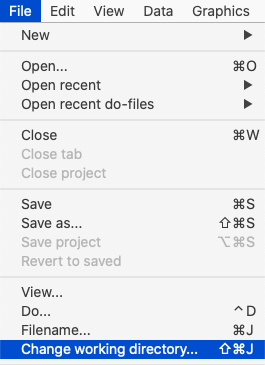
\includegraphics[scale=0.3]{image/cwd}
	
	\end{itemize}
\end{column}
\end{columns}
	

\end{frame}

%%%%
\section{Import and save data}
\subsection{Import}
\begin{frame}[fragile]{\secname: \subsecname}
\begin{itemize}
	\item \textbf{Excel (.xls or .xlsx)} \begin{verbatim}import excel filename, clear firstrow \end{verbatim}
	\item \textbf{Delimited (.csv) or text (.txt)} 
		\begin{verbatim}import delimited filename, clear
infile filename, clear\end{verbatim}
	\item \textbf{Stata (.dta)} \begin{verbatim}use filename, clear \end{verbatim}
	\item \textbf{SAS (.xpt)} \begin{verbatim}fdause filename, clear \end{verbatim}
\end{itemize}
\end{frame}

%%%
\subsection{Save}
\begin{frame}[fragile]{\secname: \subsecname}
\begin{itemize}
\item Save your dataset as a Stata file \verb|.dta|
\item The \verb|replace| option lets you overwrite the existing dataset.
\begin{verbatim}
save "filename", replace
\end{verbatim} 
\end{itemize}
\end{frame}


%%
%%%%
\section{Manage datasets}
\subsection{Merge}
\begin{frame}[fragile]{\secname : \subsecname}
\verb|merge| adds new variables from a second dataset to your existing dataset.
(Make the dataset wider)\\[4mm]
\small
\begin{verbatim}

. sysuse cancer, clear
(Patient Survival in Drug Trial)

. gen id = _n 

. keep id

. merge 1:1 id using cancer 

    Result                           # of obs.
    -----------------------------------------
    not matched                             0
    matched                                48  (_merge==3)
    -----------------------------------------

\end{verbatim}
\end{frame}

%%%%
\subsection{Append}
\begin{frame}[fragile]{\secname : \subsecname}
\verb|append| adds new observations to existing variables in your current dataset. \\ (Make the dataset longer) \\[4mm]
\small
\begin{verbatim}
. use cancer_drug12, clear 
(Patient Survival in Drug Trial)

. append using cancer_drug3.dta // append patients using drug 3
\end{verbatim}
\end{frame}

%%

\section{Get to know the data}
\subsection{Summarize}
\begin{frame}[fragile]{\secname : \subsecname}
\verb|summarize| gives summaries for all your variables, such as number of observations, mean, standard deviation, etc. \\[4mm]
\scriptsize
\begin{verbatim}
. sysuse cancer, clear
(Patient Survival in Drug Trial)

. keep if drug ==1 | drug == 2
(14 observations deleted)

. summarize age  // One variable only (age)

    Variable |        Obs        Mean    Std. Dev.       Min        Max
-------------+---------------------------------------------------------
         age |         34    56.41176    6.010686         47         67

	
\end{verbatim}

\end{frame}

%%%%

\subsection{Describe}
\begin{frame}[fragile]{\secname : \subsecname}
\verb|describe| gives descriptions for all your variables, such as storage type and labels. \\[4mm]
\scriptsize
\begin{verbatim}
. describe  age 

              storage   display value
variable name   type    format  label variable label
-------------------------------------------------------------------
age             byte    %8.0g         Patient's age at start of exp.


\end{verbatim}

\end{frame}

%%%%
\subsection{Codebook}
\begin{frame}[fragile]{\secname : \subsecname}
\verb|codebook| is a combination of \verb|summarize| and \verb|describe| and will give a detailed summary of all your variables, including mean, sd, range, percentiles, missing, frequency, etc. \\[4mm]
\tiny
\begin{verbatim}
. codebook  age

---------------------------------------------------------------------------------------------------------------------
age                                                                      Patient's age at start of exp.
---------------------------------------------------------------------------------------------------------------------

                  type:  numeric (byte)

                 range:  [47,67]                      units:  1
         unique values:  15                       missing .:  0/34

                  mean:   56.4118
              std. dev:   6.01069

           percentiles:        10%       25%       50%       75%       90%
                                49        51        56        61        65

\end{verbatim}
\end{frame}

%%%%
\subsection{List}
\begin{frame}[fragile]{\secname : \subsecname}
\verb|list| lists the observations of specified variables. \\[4mm]
\small
\begin{verbatim}
. list      age if age < 50

     +-----+
     | age |
     |-----|
 12. |  49 |
 15. |  49 |
 18. |  49 |
 25. |  49 |
 33. |  47 |
     +-----+

\end{verbatim}
\end{frame}


%%%%
\section{Manage variables}
\subsection{Numeric and string}
\begin{frame}[fragile]{\secname : \subsecname}
\begin{itemize}
\item \textbf{Numeric variables}: have values that are numbers \\
\item \textbf{String variables}: have variables that contain not just numbers
\item<2|handout:2>[] \begin{verbatim}
// Make age (numeric) into a string variable.
tostring age, replace
// convert string into numeric
destring age, replace	
 \end{verbatim}

\end{itemize}
\end{frame}

%%% 
\subsection{Drop/Keep}
\begin{frame}[fragile]{\secname : \subsecname}
\begin{itemize}
	\item \verb|drop| is used to delete variables or observations.
	\item \verb|keep| is used to keep variables or observations.
\end{itemize}

\small
\begin{verbatim}
. sysuse cancer, clear
(Patient Survival in Drug Trial)
. drop if drug ==1 | drug == 2
(34 observations deleted)

. sysuse cancer, clear
(Patient Survival in Drug Trial)
. keep if drug ==1 | drug == 2 // So drug == 3 will be dropped
(14 observations deleted)
\end{verbatim}
\end{frame}

%%% 
\subsection{Label}
\begin{frame}[fragile,allowframebreaks]{\secname : \subsecname}
\begin{itemize}
	\item 	\verb|label| helps you keep track of your dataset and variables, and helps others understand your data. 
\end{itemize}

\footnotesize
\begin{verbatim}
. // Label a dataset
. label data "cancerdata" 
\end{verbatim}
\begin{center}
	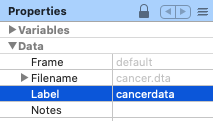
\includegraphics[scale=0.5]{image/label_data}
\end{center}

\begin{verbatim}
. // Label variable in the "Variables" window
. label variable drug "1=placebo, 2=mild, 3=strong"
\end{verbatim}

\begin{center}
	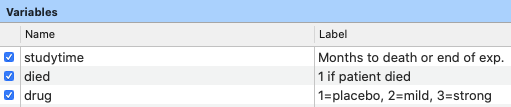
\includegraphics[scale=0.4]{image/label_var}
\end{center}

\framebreak

\begin{verbatim}
. // Label define claims the value label
. label define drug_label 1 "placebo" 2 "mild" 3 "strong"

. // Label value then assigns the label to the variables
. label values drug drug_label
\end{verbatim}

\begin{center}
	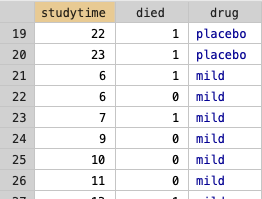
\includegraphics[width=50mm,scale=0.5]{image/label_def}
\end{center}

\end{frame}

%%% 
\subsection{Rename, recode, generate, replace}
\begin{frame}[fragile]{\secname : \subsecname}
\begin{itemize}
\item 	\verb|rename| changes the name of a variable. 
\item[] \verb|. rename died death|
\item   \verb|recode| changes variable values.
\item[] \verb|. recode drug (3=4)|
\item   \verb|generate| creates a new variable.
\item[] \verb|. generate placebo = 1 if drug == 1|
\item   \verb|replace| replaces existing variables (or variable values).
\item[] \verb|. replace placebo = 0 if drug != 1|
\end{itemize}
\end{frame}

%%% 
\subsection{Sort, by, if, in}
\begin{frame}[fragile]{\secname : \subsecname}
\begin{itemize}
	\item \verb|sort| orders observations in ascending order.\\
\begin{verbatim}
. sort death
\end{verbatim}
	\item \verb|by| executes a command within a specified variable (e.g. by age group), but data should be sorted first.
\begin{verbatim}
. by death: summarize
\end{verbatim}
	\item \verb|bysort| combines the by and sort commands into one.
\begin{verbatim}
. bysort death: summarize // by death, sort: summarize
\end{verbatim}
	\item \verb|if| is used to select by a condition.
\begin{verbatim}
. list age if death == 1
\end{verbatim}	

\item \verb|in| is used to select by observations.
\begin{verbatim}
. gen id = _n 
. list id 1/10
\end{verbatim}
\end{itemize}
\end{frame}

%%% 
\subsection{Operators}
\begin{frame}[fragile]{\secname : \subsecname}
\small
\renewcommand{\arraystretch}{1.25}
\begin{tabulary}{\textwidth}{LLL}
    \toprule
    \textbf{Operator} & \textbf{Purpose} & \textbf{Example} \\
    \midrule
    =  & Sets equal operator & generate sex = 1 \\
    == & Tests for equality & summarize if sex==1 \\
    $\sim$= or != & Indicates `not equal' & summarize if sex!=0 \\
    $< , <= \newline > , >=$ & Less than (equal to) or greater than (equal to) & summarize if age$<$35 \\
    \& & Indicates `and' & summarize outcome if sex==1 \& age$>=$60 \\
    $ \mid $ & Indicates `or' & gen x=1 if a==1 \& \newline (b==1 $\mid$ c==1) \\
\end{tabulary}
\end{frame}

%%%
\section{References}
\begin{frame}[allowframebreaks,fragile]{\secname}
    \begin{scriptsize}
	\bibliographystyle{../bib/vancouv12}
	\bibliography{../bib/enochref.bib}
    \end{scriptsize}
\end{frame}

\end{document}